\documentclass[12pt,twoside]{book}

\listfiles % create a listing in the log of all needed files

%====================================================================
% LaTeX packages
%====================================================================
\usepackage{csquotes}
\usepackage{mathtools} % Provides multlined environment
\usepackage{caption}
\captionsetup{format=hang, margin=10pt, font=small, labelfont=bf}
\usepackage{graphicx}
\usepackage{makeidx}
\usepackage{amsmath,amsfonts,amssymb,physics}
\usepackage{xcolor}
\usepackage[bookmarks=true]{hyperref}

\usepackage{booktabs}
\usepackage{geometry}
\usepackage{array}

\definecolor{linkscolor}{rgb}{0.36,0.54,0.66}
\hypersetup{
  colorlinks=true,
  linkcolor=linkscolor,
  urlcolor=linkscolor,
  citecolor=linkscolor,
  pdfauthor={Yeray Cruz Ruiz},
  pdftitle={Active Bath},
  pdfsubject={Master Thesis},
  pdfkeywords={soft matter, statistical physics, colloidal models},
  pdfproducer={LaTeX},
  pdfcreator={pdfLaTeX},
}
\usepackage[english]{babel}
\usepackage{ifthen}
\usepackage{times} % font style
\usepackage{fullpage} % page size
\usepackage[numbers,sort&compress]{natbib}
\usepackage{tikz}
\usepackage{float}
\usepackage[colorinlistoftodos]{todonotes}
\newcommand{\inlinenote}[1]{\todo[inline]{#1}}

\makeindex % activate index-making

%====================================================================
% Formatting
%====================================================================

\headsep = 25 pt % avoid the top margin problem

% set linespace to 1.2 for readability
\renewcommand{\baselinestretch}{1.2}

% Reset page margins properly for doublesided pages
\setlength{\marginparwidth}{0pt}
\setlength{\marginparsep}{0pt}
\setlength{\oddsidemargin}{0.125in}
\setlength{\evensidemargin}{0.125in}
\setlength{\textwidth}{6.375in}
\raggedbottom

%====================================================================
% Custom commands
%====================================================================

\newcommand{\e}{\mathrm{e}}
\newcommand{\kb}{k_{B}}

\newenvironment{where}[1]   % Equation symbol lists
 {\begin{list}{}%
  {\renewcommand{\makelabel}[1]{\hfill\textnormal{##1 =}}%
   \settowidth{\labelwidth}{\textnormal{#1 =}}%
   \setlength{\leftmargin}{\labelwidth}%
   \addtolength{\leftmargin}{\labelsep}%
   \setlength{\itemsep}{-\parsep}}}%
 {\end{list}}

%====================================================================
% Document
%====================================================================

\begin{document}
%----- FRONT MATERIAL -----%

\pagenumbering{roman}

\thispagestyle{empty} % No headers or page numbers

\begin{center}
\large { Instituto Tecnológico y de Estudios Superiores de Monterrey\\}
\vspace*{0.5em}
\normalsize { Campus Monterrey } \\
\vspace*{0.5em}
\large{School of Engineering and Sciences\\}
\vspace*{1em}

\begin{figure}[!h]
 \begin{center}
  
\includegraphics[scale=0.2]{pics/LogoTec.jpg}
 \end{center}
\end{figure}
\vspace*{0.6cm}

\Large {Induced Rotation of Ratchets in Passive Environments}

\vspace*{0.5em}
\normalsize{A thesis presented by}\\
\vspace*{0.5em}
\large{Yeray Cruz Ruiz}\\
\vspace*{1.5cm}
\normalsize

Submitted to the\\
School of Engineering and Sciences\\
in partial fulfillment of the requirements for the degree of\\
\vspace*{1em}
\large{Master} \\
\large{In} \\
\large{Nanotechnology} \\
\normalsize
\vfill
Monterrey, Nuevo León, México, Nov 2025\\
\end{center}

\newpage %-------------------------------------------- -----------------PAGE iii

\begin{center}

\large { Instituto Tecnológico y de Estudios Superiores de Monterrey\\}
\normalsize {Campus Monterrey}
\normalsize {School of Engineering and Sciences}
\vspace*{1em}

The commitee members, hereby, certify that have read the thesis presented by {\bf Yeray Cruz Ruiz} and that it is fully adequate in scope and quality as a partial requirement for the degree of Master in Nanotechnology.\\
\vspace*{3em}

\raggedleft{
{---------------------------------} \\
Antonio Ortiz Ambriz, PhD \\
Thesis Advisor\\
School of Engineering Sciences, Tecnológico de Monterrey\\
\vspace*{2em}
{---------------------------------}\\
Someone, PhD  \\
Sinodal member  \\
Affiliation\\
\vspace*{2em}
{---------------------------------}\\
Someone, PhD  \\
Sinodal member  \\
Affiliation\\
\vspace*{2em}
{---------------------------------}\\
Someone, PhD  \\
Sinodal member  \\
Affiliation\\
\vspace*{2em}
}

\center{
\vfill
{--------------------------------------------------} \\
Dr. Elisa Virginia Vázquez Lepe\\
Graduate Studiates Director\\
School of Engineering and Sciences}\\
Monterrey, Nuevo León, México, May 2025
\end{center}

\newpage %------------------------------------------PAGE iv

\begin{center}
\bf{Declaration of Authorship}
\end{center}

I, Yeray Cruz Ruiz (student), declare that this thesis titled, \enquote{Induced Rotation of Ratchets in Passive Environments} and the work presented in it are my own. I confirm that:

\begin{itemize}
  \item This work was done wholly or mainly while in candidature for a research degree at this University.
  \item Where any part of this thesis has previously been submitted for a degree or any other qualification at this University or any other institution, this has been clearly stated.
  \item Where I have consulted the published work of others, this is always clearly stated.
  \item Where I have quoted from the work of others, the source is always given. Apart from such quotations, this thesis is entirely my own work.
  \item I have acknowledged all main sources of help.
  \item Where the thesis is based on work done by myself jointly with others, I have made clear exactly what was done by others and what I have contributed myself.
\end{itemize}

\vspace{5em}

\begin{flushright}
{-------------------------------------------------} \\
Yeray Cruz Ruiz (Student) \\
Monterrey, Nuevo León, México, May 2025
\end{flushright}

\vfill
\begin{center}
\large {\copyright 2025 by Yeray Cruz Ruiz}\\
\large{All Rights reserved}
\end{center}


\newpage %------------------------------------------PAGE iv

\Huge {\bf Dedication}

\vfill
\normalsize To my parents for their unwavering support, to my friends for making this journey easier, and especially to Dr. Antonio, who always believed in me and was an incredible mentor. 
\vfill


\newpage %------------------------------------------PAGE vi
\Huge {\bf Acknowledgements} \\
\normalsize

For those who come after.

\vspace{5em}

\newpage %------------------------------------------PAGE vii
\begin{center}
  \large {{\bf Induced Rotation of Ratchets in Passive Environments}\\
  by\\
Yeray Cruz Ruiz}
\end{center}
\addcontentsline{toc}{chapter}{Abstract}
\Huge{{\bf Abstract}} \\
\normalsize
\vspace*{0em}

Swimming at the mesoscale has been a topic of interest for the past two decades because of the complexity of motion at a low Reynolds number, a regime where the viscous forces dominate over the inertial ones. The scallop theorem is a principle that follows these complex ideas and states that a scallop, which has only one degree of freedom, must be unable to have net displacement in this regime due to the lack of time-reversal symmetry of the Navier-Stokes equations. Indifferent to our mathematical understanding, nature was capable of creating biological beings that are able to displace under these circumstances by developing what we call nonreciprocal motion. The esquerichia coli, for example, has a flagellum that rotates in one direction, pushing the fluid backwards and therefore moving the bacteria forwards. Inspired by these ideas, researcher have taken interest in generating motion at those scales. One example are bacterial micromotors, where a dented ratchet is immersed into a bacterial bath where they convert energy from their surroundings into movement. This movement normally follows a ballistic trajectory and in time some of them, will collide into the ratchet transferring their kinetic energy, and therefore making the motor spin thanks to the geometry of the ratchet. Unfortunately, the nutrients they absorb will end and in time the system's medium will need to be replaced, stopping the whole process, therfore being an inneficient process. This is a type of active matter that gets energy from its medium. But, Can we do the same with passive matter?

In this work, we analsze paramagnetic colloids, manipulated by an external precessing magnetic field. The system is confined betwen the \textit{z} axis and presents periodic boundary conditions in \textit{x}, and \textit{y} axis. When multiple particles are present, dipole-dipole interactions arise, leading to either attraction or repulsion depending on their head-to-tail alignment. The particles' internal fields also rotate, dynamically altering their interactions over time. We observe that from 0Hz to 3Hz, the colloids form pairs and start rotating with a shared center of mass, whereas from 3.25 to 7Hz particles have a moment of replsion, creating a neighbor exchange between different pairs, obtaining a ballistic trajectorWe observe that from 0Hz to 3Hz, the colloids form pairs and start rotating with a shared center of mass, whereas from 3.25 to 7Hz particles have a moment of replsion, creating a neighbor exchange between different pairs, obtaining a ballistic trajectory. To investigate whether this motion can perform work, we place a ratchet-like object with different parameters amidst the particles.

\newpage %-------------------------------------------PAGE viii

\listoffigures
\addcontentsline{toc}{chapter}{List of Figures}

\listoftables
\addcontentsline{toc}{chapter}{List of Tables}

% \listoffigures
% \listoftables
\tableofcontents
\newpage

\pagenumbering{arabic} % Change page numbering back to Arabic numerals


\pagenumbering{arabic}
%----- MAIN BODY -----%

% Put the document title and page numbers in the header
\pagestyle{myheadings}
\normalsize

% Chapters



\part{Introduction}
\label{part:introduction}

%======================================================================
\chapter{Introduction}
\label{ch:introduction}

\markright{Introduction}
%======================================================================
The study of motion at the microscale sits between physics, chemistry, and biology, and has consequences both for basic science and for applications. At these scales, inertia can be ignored and viscous forces dominate. Random fluctuations from thermal noise also play an important role. How to control, rectify, and use this motion is one of the main questions in soft matter and statistical physics~\cite{purcell2014life,einstein1906theory}. Besides the theoretical interest, these ideas are useful for the design of microfluidic devices, targeted drug delivery, and even nanoscale engines.

Nature already provides many examples of how small systems can turn energy into motion. Inside cells, molecular motors like kinesin and dynein move cargo. Microorganisms such as \textit{E. coli}, sperm cells, and algae have developed strategies to swim in viscous environments~\cite{howard2002mechanics, vale2003molecular, marchetti2013hydrodynamics}. These observations gave rise to the field of \textit{active matter}, which studies collections of self-driven units operating out of equilibrium~\cite{ramaswamy2010mechanics, needleman2017active, bechinger2016active}. The concept has expanded in recent years to cover emergent effects, such as topological flows in active materials~\cite{shankar2022topological}.

One useful way to think about directed motion at this scale is through ratchets. These are asymmetric structures or potentials that turn random fluctuations into net motion, similar to Feynman’s ratchet thought experiment. Ratchets have been studied in both theory and experiments, leading to the broader field of Brownian motors~\cite{julicher1997modeling, reimann2002brownian}. More recently, these ideas have been extended to active matter, where active Brownian particles can be rectified into directional transport~\cite{fiasconaro2008active, reichhardt2017ratchet, rein2023force}.

Di Leonardo \textit{et al.} (2010) harnessed the movement of living cells and showed that asymmetric microgears immersed in dense bacterial suspensions could rotate spontaneously, powered only by the activity of \textit{E. coli}~\cite{di2010bacterial}. These bacterial ratchets combine nonequilibrium activity with geometric asymmetry to produce motion. Such systems point to possible uses in autonomous transport and mixing at the microscale. Also it has been studied how bacterium collisions with curved-geometry microstructures can exert net movement in these structures and how the curvature of the surface can modify the speed of the structure~\cite{pellicciotta2025wall}.

Even with these advances, there are still open problems. Active matter is powerful but not always easy to control or keep stable, since living systems depend strongly on their environment~\cite{bechinger2016active}. Passive colloids are easier to handle in experiments but need external driving to move in a directed way. Magnetically driven colloids are promising in this respect because their interactions can be tuned, they are reversible, and they can be controlled externally. Experiments have shown magnetic colloidal carpets that propel and carry cargo~\cite{martinez2015magnetic}, and other studies have revealed enhanced diffusion, synchronization, and bidirectional transport under confinement~\cite{tierno2012depinning, straube2014tunable, ostinato2024magnetically}. Still, the interplay between confinement, collective effects, and external driving is not fully understood.

This thesis looks at these questions by using numerical simulations of paramagnetic colloids under magnetic fields, with emphasis on confinement and ratchet effects. Simulations are useful because they allow us to test conditions that are hard to achieve in experiments and to separate the roles of noise, interactions, and driving. By studying transport properties, collective effects, and symmetry breaking, we aim to clarify how random microscopic motion can be rectified into useful work. The results connect to basic questions in nonequilibrium systems and may also guide the design of micro- and nanoscale devices, where controlled transport is essential.

The thesis is organized as follows. Part~\ref{part:background} reviews the theoretical background, including motion at low Reynolds number, Brownian noise, ratchet mechanisms, and the difference between active and passive matter. Part~\ref{part:methods} describes the simulation methods, with focus on stochastic molecular dynamics. Part~\ref{part:results} presents the main findings on confined colloidal dynamics and rectification. Finally, Part~\ref{part:conclusions} summarizes the contributions and suggests future work.
 \newpage




\part{Background}
\label{part:background}

%======================================================================
\chapter{Physics at the mesoscale}
\label{ch:swimming at the mesoscale}

\markright{Swimming at the mesoscale}
%======================================================================

\section{Low Renolds number regime}
\label{st:lowreynoldsnumber}

At the mesoscale, where objects such as bacteria and colloidal particles operate, the physical world is governed by a regime in which viscous forces dominate over inertial ones. This regime is characterized by a small Reynolds number (Re), a dimensionless quantity that compares inertial to viscous effects. Therefore, the force applied at that moment will describe the movement or displacement performed, not deppending on any past force, this is a characteristic of an overdamped system. In his seminal lecture, Life at Low Reynolds Number, Purcell highlighted the surprising and often counterintuitive behaviors that emerge in such environments \cite{purcell2014life}. For instance, time-reversible motion — common at macroscopic scales — is ineffective for propulsion at low Re, necessitating non-reciprocal strategies like flagellar rotation or body undulation. This leads to the scallop theorem, that states that an animal with such degrees of freedom — in a viscous regime — will not have a net displacement. 

This whole process can be described by the Navier-Stokes equation without the inertia terms, leaving us without any time deppending terms as shown in \ref{eq:Navier-Stokes}. 

\begin{equation}
  - \nabla p + \eta \nabla ^2 \vec{v} = 0
  \label{eq:Navier-Stokes}
\end{equation}

This has been a topic of interest for researchers that are constantly looking for ways of transportation in those environments for specific tasks. Unfortunately this is not the only challenge we face when moving at the microscale.

\section{Brownian Motion and Thermal Fluctuations}
\label{st:brownianmotion}

Even though this is a viscous regime, particles are not static. At small length scales, such as those of colloidal particles or bacteria, random thermal fluctuations become a dominant source of motion. This phenomenon, known as \textit{Brownian motion}, was first explained quantitatively by Albert Einstein in 1905. He demonstrated that the irregular paths observed in microscopic particles suspended in fluid result from collisions with the molecules of the surrounding medium~\cite{einstein1906theory}.

Einstein's work provided one of the first convincing arguments for the molecular nature of matter and led to a mathematical description of how these random movements accumulate over time. Specifically, he derived that the mean squared displacement (MSD) of a particle grows linearly with time:

\begin{equation}
  \langle x^2(t) \rangle = 2Dt\text{,}
  \label{eq:msd}
\end{equation}

where $D$ is the diffusion coefficient, a measure of how quickly particles spread out. Einstein further related this coefficient to measurable physical parameters through the expression:

\begin{equation}
  D = \frac{k_{B}T}{6\pi \eta R}\text{,}
  \label{eq:diffusioncoefficient}
\end{equation}

where $k_B$ is Boltzmann’s constant, $T$ the absolute temperature, $\eta$ the dynamic viscosity of the fluid, and $R$ the radius of the spherical particle. This relation — often referred to as the \textit{Einstein-Stokes equation} — is foundational in soft matter and colloidal physics.

In the systems considered in this thesis, Brownian motion plays a crucial role in the dynamics of passive colloids and must be accounted for even in the presence of external fields or active agents, such as bacteria.

\vspace{1em}

While Einstein’s formulation captures the long-term diffusive behavior of Brownian particles, it does not account for their instantaneous dynamics. To describe how particles move under both viscous damping and random thermal forces, we turn to a stochastic differential equation known as the \textit{Langevin equation}.

\subsection{Stochastic Representation}

The Langevin equation \cite{uhlenbeck1930theory} in one dimension, including inertial effects, damping, and thermal noise, can be written as:

\begin{equation}
  m\ddot{x} = F - \lambda \dot{x} + \eta(t)\text{,}
  \label{eq:newton}
\end{equation}

where $m$ is the particle mass, $\lambda$ is the damping coefficient, and $\eta(t)$ is a stochastic force representing thermal noise. For simplicity, we write the velocity as $v = \dot{x}$, leading to:

\begin{equation}
  m\frac{dv}{dt} = F - \lambda v + \eta(t)\text{.}
  \label{eq:newtonv}
\end{equation}

Discretizing time with a small step $dt$, we apply the definition of a derivative:

\begin{equation}
  m \frac{v(t + dt) - v(t)}{dt} = F - \lambda v(t) + \eta(t)\text{.}
  \label{eq:newtonderivative}
\end{equation}

The thermal noise term $\eta(t)$ is modeled as a Gaussian white noise process:

\begin{equation}
  \eta(t)\, dt = g\, dW\text{,}
  \label{eq:eta}
\end{equation}

where $dW$ is a Wiener process (increment of Brownian motion) such that:

\begin{equation}
  \langle dW \rangle = 0\,, \quad \langle dW^2 \rangle = dt\text{.}
  \label{eq:meanvariance}
\end{equation}

Solving for $v(t + dt)$ gives:

\begin{equation}
  v(t + dt) = v(t) + \frac{dt}{m}(F - \lambda v(t)) + g\, dW\text{.}
  \label{eq:velocityplusone}
\end{equation}

Now, assuming no deterministic force ($F = 0$) — as is the case for free passive particles:

\begin{equation}
  v(t + dt) = v(t) - \frac{\lambda dt}{m} v(t) + g\, dW\text{.}
  \label{eq:noforce}
\end{equation}

Taking the expectation value (mean) of both sides:

\begin{equation}
  \langle v(t + dt) \rangle = \langle v(t) \rangle - \frac{\lambda dt}{m} \langle v(t) \rangle + g \langle dW \rangle\text{.}
  \label{eq:mean}
\end{equation}

Since $\langle dW \rangle = 0$, the last term vanishes:

\begin{equation}
  \langle v(t + dt) \rangle = \langle v(t) \rangle \left( 1 - \frac{\lambda dt}{m} \right)\text{.}
\end{equation}

In the limit of small $dt$, this leads to the differential equation:

\begin{equation}
  \frac{d}{dt} \langle v(t) \rangle = - \frac{\lambda}{m} \langle v(t) \rangle\text{,}
  \label{eq:derivative}
\end{equation}

whose solution is:

\begin{equation}
  \langle v(t) \rangle = \langle v(0) \rangle\, e^{-\lambda t / m}\text{.}
\end{equation}

This result shows that the average velocity of a particle in a viscous fluid decays exponentially due to damping. The characteristic timescale $\tau = m/\lambda$ describes how quickly the particle forgets its initial velocity, after which the motion becomes diffusive.

%%%%

\subsection{Velocity Statistics and Energy Equipartition}

To compute the variance of the velocity, we start again from the Langevin equation in discretized form, without external forces:

\begin{equation}
  v(t + dt) = v(t) - \frac{\lambda}{m} v(t) dt + \frac{g}{m} dW \text{.}
\end{equation}

Squaring both sides:

\begin{align}
  v(t + dt)^2 &= \left[ v(t) - \frac{\lambda}{m} v(t) dt + \frac{g}{m} dW \right]^2 \text{,}\\
              &= v(t)^2 + \left( \frac{\lambda}{m} \right)^2 v(t)^2 dt^2 + \left( \frac{g}{m} \right)^2 dW^2 \nonumber \\
              &\quad - 2 \frac{\lambda}{m} v(t)^2 dt + 2 \frac{g}{m} v(t) dW - 2 \frac{\lambda g}{m^2} v(t) dW \text{.}
\end{align}

Now we take the expectation value:

\begin{align}
  \langle v(t + dt)^2 \rangle &= \langle v(t)^2 \rangle + \left( \frac{\lambda}{m} \right)^2 \langle v(t)^2 \rangle dt^2 + \left( \frac{g}{m} \right)^2 \langle dW^2 \rangle \nonumber \\
                              &\quad - 2 \frac{\lambda}{m} \langle v(t)^2 \rangle dt + 2 \frac{g}{m} \langle v(t) \rangle \langle dW \rangle - 2 \frac{\lambda g}{m^2} \langle v(t) \rangle \langle dW \rangle \text{.}
\end{align}

Using the properties of the Wiener process:

\[
  \langle dW \rangle = 0, \quad \langle dW^2 \rangle = dt \text{.}
\]

And neglecting second-order small terms (\( dt^2 \)), we obtain:

\begin{equation}
  \langle v(t + dt)^2 \rangle = \langle v(t)^2 \rangle + \frac{g^2}{m^2} dt - 2 \frac{\lambda}{m} \langle v(t)^2 \rangle dt \text{.}
\end{equation}

Taking the continuous limit:

\begin{equation}
  \frac{d}{dt} \langle v(t)^2 \rangle = -2 \frac{\lambda}{m} \langle v(t)^2 \rangle + \frac{g^2}{m^2} \text{.}
\end{equation}

This is a linear first-order ODE. Solving it with variation of constants yields:

\begin{equation}
  \langle v(t)^2 \rangle = \frac{g^2}{2 \lambda m} + D e^{-2 \lambda t / m} \text{.}
\end{equation}

As \( t \to \infty \), the exponential term vanishes and we get the stationary value:

\begin{equation}
  \langle v(\infty)^2 \rangle = \frac{g^2}{2 \lambda m} \text{.}
\end{equation}

From the equipartition theorem, we know that the average kinetic energy is:

\[
  \frac{1}{2} m \langle v^2 \rangle = \frac{1}{2} k_B T \text{.}
\]

Therefore:

\begin{equation}
  \langle v^2 \rangle = \frac{k_B T}{m} \text{.}
\end{equation}

Matching this to our stochastic result:

\begin{equation}
  \frac{k_B T}{m} = \frac{g^2}{2 \lambda m} \quad \Rightarrow \quad g^2 = 2 \lambda k_B T, \quad g = \sqrt{2 \lambda k_B T} \text{.}
\end{equation}

This defines the noise amplitude in terms of temperature, viscosity, and Boltzmann’s constant.

\subsection{Overdamped Dynamics and Diffussion}

In the overdamped limit, inertia is negligible, so the Langevin equation becomes:

\begin{equation}
  0 = F - \lambda \frac{dx}{dt} + \eta(t) \text{.}
\end{equation}

Solving for the velocity:

\begin{equation}
  \frac{dx}{dt} = \frac{1}{\lambda} (F + \eta(t)) \text{.}
\end{equation}

For free diffusion (\( F = 0 \)):

\begin{equation}
  \frac{dx}{dt} = \frac{1}{\lambda} \eta(t) \text{.}
\end{equation}

Using stochastic calculus with \( \eta(t) dt = g dW \), we write:

\begin{equation}
  x(t + dt) = x(t) + \frac{g}{\lambda} dW \text{.}
\end{equation}

\paragraph{Mean Position}

Taking the expectation:

\begin{equation}
  \langle x(t + dt) \rangle = \langle x(t) \rangle + \frac{g}{\lambda} \langle dW \rangle = \langle x(t) \rangle \text{.}
\end{equation}

So the mean position remains constant in free diffusion.

\paragraph{Mean Square Displacement (MSD)}

Squaring the position update:

\begin{equation}
  x(t + dt)^2 = x(t)^2 + 2 \frac{g}{\lambda} x(t) dW + \left( \frac{g}{\lambda} \right)^2 dW^2 \text{.}
\end{equation}

Taking the expectation:

\begin{align}
  \langle x(t + dt)^2 \rangle &= \langle x(t)^2 \rangle + 2 \frac{g}{\lambda} \langle x(t) \rangle \langle dW \rangle + \frac{g^2}{\lambda^2} \langle dW^2 \rangle \text{,}\\
  &= \langle x(t)^2 \rangle + \frac{g^2}{\lambda^2} dt \text{.}
\end{align}

In differential form:

\begin{equation}
  \frac{d}{dt} \langle x(t)^2 \rangle = \frac{g^2}{\lambda^2} \text{.}
\end{equation}

Using \( g^2 = 2 \lambda k_B T \), we substitute:

\begin{equation}
  \frac{d}{dt} \langle x(t)^2 \rangle = \frac{2 k_B T}{\lambda} \text{.}
\end{equation}

Integrating gives the mean squared displacement (MSD):

\begin{equation}
  \langle x(t)^2 \rangle = \frac{2 k_B T}{\lambda} t \text{.}
\end{equation}

This is the classical diffusion result, where the diffusion coefficient is \( D = \frac{k_B T}{\lambda} \), consistent with Einstein's expression.



%%%%
%This raises a fundamental question: Can these fluctuations be harnessed to perform useful work? This idea lies at the heart of thought experiments such as the Feynman ratchet, which challenge our understanding of thermodynamics at microscopic scales.


\begin{figure}[H]
  \begin{center}
    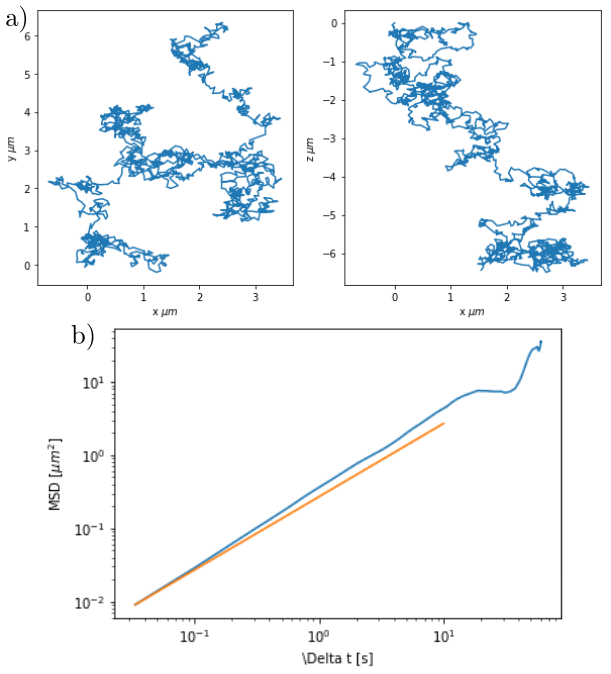
\includegraphics[width=0.8\textwidth]{figures/passivebrowniantrajectorymsd.png}
  \end{center}
  \caption[Example of brownian motion]{A colloidal particle undergoes random, thermally induced displacements in a fluid medium. \textbf{Panel a)} shows the trajectory of the particle. \textbf{ Panel b)} shows the corresponding mean squared displacement (MSD) as a function of time, illustrating the linear relationship predicted by Einstein for diffusive behavior (orange) and the one obtained through a numerical simulation (blue).}\label{fig:passivebrowniantrajectory}
\end{figure}

\chapter{Ratchets and Rectification Mechanisms}
\label{ch:ratchetsandrectificationmechanisms}

\section{The Feynman-Smoluchowski ratchet}

The inherent randomness of Brownian motion naturally leads to the question: can this disorder be transformed into order? In other words, can the random thermal motion of particles be used to produce directed movement or extract work? This question sits at the core of statistical mechanics and was famously explored by Richard Feynman in his lectures on physics, through a thought experiment known as the Feynman ratchet and pawl \cite{feynman1963feynman}.

The Feynman ratchet consists of a set of vanes connected to a ratchet wheel, immersed in a fluid (Fig. \ref{fig:feynmanratchet}). The idea is: random collisions from the surrounding molecules could push the vanes, but the pawl only allows rotation in one direction. At first glance, this asymmetric mechanism seems capable of converting random thermal motion into unidirectional rotation, apparently violating the second law of thermodynamics.

\begin{figure}
  \begin{center}
    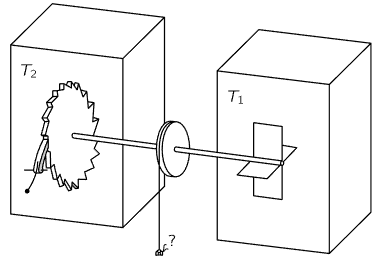
\includegraphics[width=0.65\textwidth]{figures/feynmanratchet.png}
  \end{center}
  \caption[Feynman ratchet]{Visual representation of the Feynman ratchet. Obtained from \cite{feynman1963feynman}}\label{fig:feynmanratchet}
\end{figure}


However, Feynman's analysis showed that when both the ratchet and the pawl are in thermal equilibrium with the same heat bath, the system cannot produce net work. The pawl itself undergoes thermal fluctuations and can occasionally lift off, allowing the ratchet to move backward. Over time, the forward and backward movements average out, and no net rotation occurs. This result reinforces the principle that thermal fluctuations alone cannot be rectified to perform work without a temperature gradient or an external energy input.

\begin{table}[ht]
\centering
\renewcommand{\arraystretch}{1.4}
\caption[Summary of operation of ratchet and pawl.]{Summary of operation of ratchet and pawl. Obtained from \cite{feynman1963feynman}}
\label{tab:ratchet_pawl}
\begin{tabular}{>{\itshape}l l l}
\toprule
\textbf{Forward:} & Needs energy & $\epsilon + L \theta$ from vane. \quad $\therefore$ Rate = $\dfrac{1}{\tau} e^{-(L\theta + \epsilon)/kT_1}$ \\
                  & Takes from vane & $L\theta + \epsilon$ \\
                  & Does work & $L\theta$ \\
                  & Gives to ratchet & $\epsilon$ \\
\midrule
\textbf{Backward:} & Needs energy & $\epsilon$ for pawl. \quad $\therefore$ Rate = $\dfrac{1}{\tau} e^{-\epsilon/kT_2}$ \\
                   & Takes from ratchet & $\epsilon$ \\
                   & Releases work & $L\theta$ \\
                   & Gives to vane & $L\theta + \epsilon$ \\
\bottomrule
\end{tabular}

\vspace{1em}
If system is reversible, rates are equal, hence 
\[
\frac{\epsilon + L\theta}{T_1} = \frac{\epsilon}{T_2}.
\]
\[
\frac{\text{Heat to ratchet}}{\text{Heat from vane}} = \frac{\epsilon}{L\theta + \epsilon}.
\quad \text{Hence} \quad \frac{Q_2}{Q_1} = \frac{T_2}{T_1}.
\]
\end{table}

Despite this limitation, the Feynman ratchet introduced a powerful concept: asymmetry combined with non-equilibrium conditions can, in principle, produce directed motion. This idea is foundational in the study of Brownian motors, biomolecular machines, and active matter systems, including the systems explored in this thesis. In such systems, energy is continuously supplied, whether through bacterial metabolism or magnetic field modulation, creating the necessary non-equilibrium environment that allows motion rectification to occur.

The failure of the Feynman ratchet in thermal equilibrium is intimately connected to another famous thought experiment: Maxwell's demon. Both systems attempt to extract work from thermal fluctuations through selective processes—the ratchet through mechanical asymmetry, and the demon through information gathering.

Maxwell's demon, proposed in 1867, imagines a microscopic being that can sort fast and slow molecules between two chambers, creating a temperature difference without apparent work. Similarly, the pawl in Feynman's ratchet acts as a mechanical "demon," attempting to select only forward fluctuations while blocking backward motion. However, both fail for the same fundamental reason: the cost of selection itself \cite{maxwell1871theory, maxwell1867letter}.

Brillouin (1951) and later Landauer (1961) showed that Maxwell's demon must expend energy to measure molecular velocities and erase information, with the minimum energy cost being $kT\ln{2}$ per bit erased. In the Feynman ratchet, the pawl must "decide" whether to allow motion, and this decision-making process—manifested as thermal fluctuations of the pawl itself—has an entropic cost that exactly cancels any work extracted \cite{brillouin1951maxwell, landauer1961irreversibility}.

This connection reveals a deep principle: rectification requires either an information gradient (knowledge about the system) or an energy gradient (non-equilibrium conditions). As Parrondo and Español (1996) demonstrated, the Feynman ratchet can be viewed as an information engine where the pawl performs measurements on the ratchet's position. When the pawl and ratchet are at the same temperature, the information gained equals the entropy produced, yielding no net work \cite{parrondo1996criticism}.


\section{Brownian ratchets and tilted potentials}

While Feynman's ratchet fails due to thermal equilibrium, rectified motion becomes possible when detailed balance is broken through external driving. Magnasco (1993) demonstrated this principle through the "rocking ratchet" mechanism \cite{magnasco1993forced}. In his model, a Brownian particle moves in an asymmetric periodic potential—essentially a sawtooth-shaped energy landscape with gentle slopes in one direction and steep walls in the other.
The crucial innovation was applying an oscillating force $F(t) = A\cos(\omega t)$ that rocks the potential back and forth. Although this force has zero time average—pushing equally left and right—the combination with the spatial asymmetry produces net directional motion. When the force tilts the potential forward, particles easily climb the gentle slopes and can overcome barriers. When tilted backward, particles encounter steep walls and remain trapped. This asymmetric response to symmetric driving breaks the forward-backward symmetry of thermal diffusion.

This mechanism differs fundamentally from Feynman's original ratchet: rather than attempting to rectify equilibrium fluctuations (which violates the second law), the rocking ratchet continuously injects energy through the oscillating force. The time-dependent driving maintains the system far from equilibrium, enabling the spatial asymmetry to generate directed transport. This principle—that asymmetry plus non-equilibrium driving yields rectification—underlies numerous biological processes and provides the theoretical foundation for the magnetically-driven ratchets explored in this thesis.

Following Magnasco's rocking ratchet where an oscillating force drives particles in a static potential, Ajdari et al. (1994) systematically analyzed rectification in periodic structures with either spatial or temporal asymmetry \cite{ajdari1994rectified}. Using a sawtooth potential with asymmetric slopes (steep of height $\epsilon/a$ and gentle of $\epsilon/b$), they identified distinct transport regimes as a function of the AC force amplitude $\gamma$. 

For small forces $\gamma < \epsilon/a$, particles remain trapped. In the intermediate regime $\epsilon/a < \gamma < \epsilon/b$, rectification occurs as particles can climb the gentle slope but not the steep one, yielding either integer velocities $V = n$ when particles fully relax between cycles (Regime 1), or rational velocities $V = n - 1/(m+1)$ when incomplete relaxation creates a periodic pattern over multiple cycles (Regime 2). The thresholds between these velocities form a complex "Devil's staircase" structure, as shown in their phase diagrams.

Ajdari et al. demonstrated that both spatial asymmetry (with symmetric forcing) and temporal asymmetry (with symmetric potential) can generate directed motion, and remarkably, when both asymmetries are present, they can either reinforce or cancel each other. This cancellation condition provides a direct way to measure the degree of asymmetry in experimental systems

Later, this concept was proven experimentally by Faucheux et al. (1995) who created an "optical thermal ratchet" using focused laser beams to generate the asymmetric potential, showing that even Brownian particles could be rectified \cite{faucheux1995optical}.
\section{Geometric ratchets}

Unlike energy ratchets that rely on asymmetric potentials, geometric ratchets achieve rectification through spatial asymmetry of boundaries or obstacles, particularly relevant for self-propelled particles

\chapter{Active Matter Systems}
\label{ch:activeandpassivemattersystems}

\section{Fundamentals of Active Matter}

Active matter refers to systems composed of self-driven units that continuously consume energy from their environment to propel themselves \cite{marchetti2013hydrodynamics, ramaswamy2010mechanics}. It is important to note it doesn't matter if the particles are artificial or oganic. The difference of active particles from passive ones, is that passive have mere diffusion motion, whereas active follows these stochastic differential equations accordnig to \cite{volpe2014simulation}:
\begin{align}
  \frac{d}{dt}x(t) &= v\cos{\varphi(t)} + \sqrt{2D_T}W_x,\\
  \frac{d}{dt}y(t) &= v\sin{\varphi(t)} + \sqrt{2D_T}W_y,\\
  \label{eq:activestochasticequation}
\end{align}

where $W_x$, and $W_y$ represent their corresponding Wiener process. As stated before, if 

\begin{equation}
  \lim_{v \to 0}  v\cos{\varphi(t)} + \sqrt{2D_T}W_x,
  \label{eq:limitofvelocity}
\end{equation}

then the motion is merely diffusive and the particle is characterized as brownian particle. Figure \ref{fig:msddifferentvelocities} helps visualize how  the motion varies according to their velocity. When the velocity is zero, the linear behavior of the MSD represents a diffusive behavior, whereas when it is different it is considered to be ballistic. 

\begin{figure}
  \begin{center}
    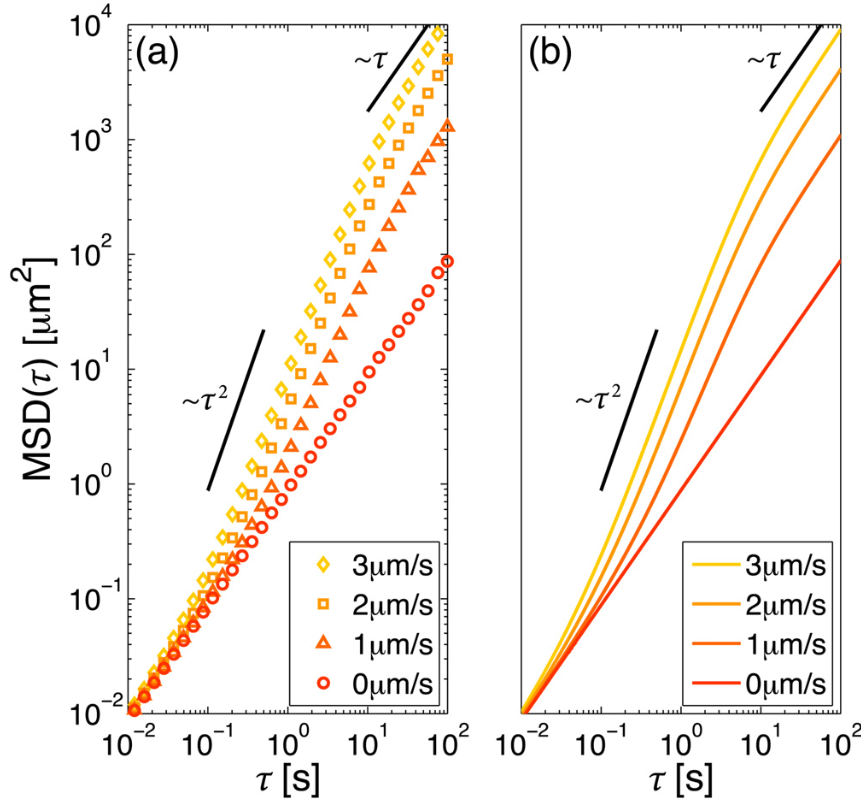
\includegraphics[width=0.55\textwidth]{figures/msddifferentvelocities.png}
  \end{center}
  \caption[MSD for passive and active brownian particles]{MSD for brownian particles with different velocites. \textbf{Panel a)} shows the result from simulations. \textbf{Panel b)} shows the theoretical calculation. Obtained from \cite{volpe2014simulation}}\label{fig:msddifferentvelocities}
\end{figure}


The foundational work by Howse et al. (2007) established the experimental basis for active Brownian particle dynamics by studying self-motile colloidal particles that use chemical reactions catalyzed on their surface to achieve autonomous propulsion. They demonstrated that at short times, these particles exhibit substantial directed motion with velocity dependent on fuel concentration, while at longer times, the motion transitions to a random walk with enhanced diffusion coefficients. This work provided the first comprehensive experimental validation of the theoretical active Brownian particle model and established the standard mathematical framework for describing such systems through coupled stochastic differential equations \cite{howse2007self}.


As discussed in section \ref{st:lowreynoldsnumber}, organisms or objects must break symmetry in specific ways to achieve net movement when swimming in environments dominated by viscous forces. Nature has evolved elegant solutions to this challenge through various biological mechanisms. A prime example is E. coli, which employs helical flagella that can rotate both clockwise and counterclockwise, generating two distinct types of motion that researchers have termed "run" and "tumble." The bacterium's response to random fluctuations also depends on the medium's viscosity \cite{kumar2010physics}.

The dynamics of active particles exhibit fascinating collective behaviors that have drawn inspiration from biological systems. A computational study by Reynolds (1987) used simulations to model flocking behavior in birds, treating each individual as an autonomous agent whose trajectory is influenced by its local environment and neighboring individuals \cite{reynolds1987flocks}. Reynolds introduced three fundamental rules governing flocking behavior: separation (collision avoidance), alignment (velocity matching with neighbors), and cohesion (attraction toward the average position of neighbors). This work established the foundation for understanding how simple local interactions can give rise to complex collective motion patterns. The principles identified by Reynolds have since been adapted and extended to describe the collective dynamics of active Brownian particles, where similar emergent behaviors such as clustering, swarming, and directed group motion arise from the interplay between self-propulsion and inter-particle interactions.

\section{Interaction with non-homogeneous environments}

All this properties considered an ideal environment, where no obstacles are present. Active particles in real environments encounter surfaces, confinement, and flow fields that dramatically alter their behavior. A striking example is the work by Hill et al. (2007), who demonstrated that E. coli swimming near surfaces in shear flow exhibit sophisticated rheotaxis - the ability to sense flow gradients and actively swim upstream through hydrodynamic surface interactions \cite{hill2007hydrodynamic}. 

\section{Active Ratchets: State of the Art}


\chapter{Magnetically Driven Colloidal Systems}
\label{magneticallydrivencolloidalsystems}

\section{Magnetic Colloids under static fields}

\section{Dynamic Magnetic Actuation}

Active matter requires a continuous source of energy to avoid falling under the category of Brownian particles. However, for complex challenges—such as transportation—these systems can tend to be inefficient due to their energy depletion.

Fortunately, Ostinato et al. (2024)
Dimer formation, exchange dynamics

Emergent currents withouth self-propulsion

In the study of motion at small scales, materials are often categorized as either active or passive. This distinction is based on whether the constituents are capable of autonomously converting energy into motion.


This thesis focuses on such externally driven passive systems, particularly on paramagnetic colloids subjected to dynamic magnetic fields. These systems provide a controlled platform to study non-equilibrium transport and rectified motion, drawing inspiration from active matter while remaining fundamentally passive in nature.

\newpage
 \newpage
\part{Methods}
\label{part:methods}

\chapter{Simulations}

The system studied in this thesis consists of an ensemble of paramagnetic colloidal particles confined in a quasi-two-dimensional geometry and subjected to an externally applied precessing conical magnetic field. Each colloid is a spherical particle of radius $r_{\mathrm{mag}}$ suspended in a Newtonian fluid of dynamic viscosity $\eta$. The suspension is bound by two parallel glass plates separated by a distance $h$, such that $h \lesssim 2R$. This strong confinement restricts particle motion primarily to two dimensions, while still allowing limited vertical displacement. 

\begin{figure}
  \begin{center}
    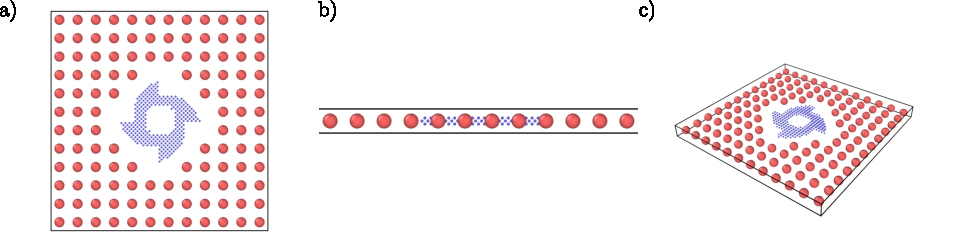
\includegraphics[width=0.95\textwidth]{figures/system.pdf}
  \end{center}
  \caption[System overview.]{System overview for a 4 spikes spin up ratchet}\label{fig:system}
\end{figure}


Numerical simulations provide a powerful framework to reproduce and analyze physical phenomena under controlled conditions. Unlike experiments, they allow for precise manipulation of initial parameters, systematic testing of hypotheses, and straightforward replication of results. In particular, simulations are invaluable when dealing with microscopic systems, where stochastic effects and complex interactions can make experimental observations challenging. 

In this thesis, numerical simulations are employed to study the dynamics of colloidal systems at the microscale. Such systems are often dominated by thermal fluctuations and many-body interactions, making them difficult to probe experimentally without advanced imaging and data analysis techniques. The primary computational approach used here is \textit{molecular dynamics} (MD), which will be described in detail in the following sections. MD enables the integration of particle trajectories under the influence of deterministic and stochastic forces, providing direct access to observables such as mean-squared displacements, velocity correlations, and transport coefficients.

\section{Molecular dynamics}



This thesis explores the physics of the system by using molecular dynamics, where randomness enters through thermal noise. As we saw in \ref{stochasticrepresentation}, the interactions can be derived from classical mechanics. In this case, Newton’s second law gives the starting point to calculate the forces acting on a single particle. In other words, at each iteration of the simulation we need to evaluate the forces that each particle experiences. Taking equation~(\ref{eq:newton}) as a starting point, and adding labels for the different interactions, we obtain:

\begin{equation}
  m_i\ddot{\vec{x_i}} = F^{collision}_i + F^{drag}_i + \eta(t)\text{,}
  \label{eq:langevinratchet}
\end{equation}
where $m_i$ is the mass of particle $i$, $\vec{x_i}$ its position, and $F^{drag}_i$ is the viscous force, written as $-\lambda \dot{\vec{x}}_i$, with $\lambda$ the drag coefficient of the fluid. Since we are working at a scale where inertial effects are negligible, the term $m_i\ddot{\vec{x_i}}$ can be dropped. The random force $\eta(t)$ represents collisions with the solvent particles. In this thesis, $\eta$ is taken as a Gaussian random force with $\expval{\eta} = 0$ and correlation $\expval{\eta_i(t)\eta_j(t')} = 2k_B T \lambda \delta_{i,j}\delta(t-t')$. This form will be used for non-paramagnetic particles.

For paramagnetic particles, we need to add the contribution of dipole–dipole interactions, which gives the modified equation:

\begin{equation}
  m_i\ddot{\vec{x_i}} = F^{collision}_i + F^{drag}_i + F^{dd}_i + \eta(t)\text{,}
  \label{eq:langevindipole}
\end{equation}
where $F^{dd}_i$ according to \cite{yung1998analytic} is described as force exerted for the dipole moment $\vec{m}_i$ on a dipole $\vec{m}_j$:

\begin{equation}
  \label{eq:dipoledipoleforce}
\vec{F}^{dd}_i = \frac{3\mu_0}{4\pi r^4}
\begin{multlined}[t]
\bigl[ (\hat{x}_{i,j} \times \vec{m}_i) \times \vec{m}_j
    + (\hat{x}_{i,j} \times \vec{m}_j) \times \vec{m}_i \\
    - 2\hat{x}_{i,j}(\vec{m}_i \cdot \vec{m}_j)
    + 5\hat{x}_{i,j}((\hat{x}_{i,j} \times \vec{m}_i) \cdot (\hat{x}_{i,j} \times \vec{m}_j)) \bigr],
\end{multlined}
\end{equation}
where $\hat{x}_{i,j}$ is the unitary vector of distance between dipoles. Since all magnetic dipoles are identical and aligned with the external magnetic field $\vec{B}_{\text{ext}}$, we can express the dipole moment as $\vec{m} = \chi V \vec{H}_{\text{ext}} = \frac{\chi V}{\mu_0} \vec{B}_{\text{ext}}$, where $\chi$ is the magnetic susceptibility and $V$ is the particle volume. Substituting $\vec{m}_i = \vec{m}_j = \vec{m}$ and expressing in terms of the external field gives:

\begin{equation}
  \label{eq:dipoledipoleforce_Bext}
  \vec{F}^{dd}_{i,j} = \frac{3\mu_0 m^2}{4\pi r^4}
\left[ 2(\hat{x}_{i,j} \times \hat{B}) \times \hat{B} - 2\hat{x}_{i,j} + 5\hat{x}_{i,j}|\hat{x}_{i,j} \times \hat{B}|^2 \right],
\end{equation}
where $m = \frac{\chi V B_{\text{ext}}}{\mu_0}$, $\hat{B} = \vec{B}_{\text{ext}}/B_{\text{ext}}$ is the unit vector along the external field, and $B_{\text{ext}} = |\vec{B}_{\text{ext}}|$. 

This is the force applied by one particle, to obtain the total dipole interaction with all particles of the system, we should add them up, pair by pair:

\begin{equation}
  F^{dd}_i = \sum^{n}_{i \neq j} F^{dd}_{i,j}.  
  \label{eq:dipolesum}
\end{equation}

We need to define the external magnetic field, which is a precessing field that forms a conical rotation of the form

\begin{equation}
  \vec{B} = B_0 [\cos{\theta}\hat{z} + \sin{\theta}\cos{(2\pi f t)}\hat{x} + \sin{(2\pi f t)}\hat{y}],
  \label{eq:magneticfield}
\end{equation}


where $B_0$ is the amplitude and $f$ the frequency of rotation of the magnetic field. The frequency plays an important role in the system dynamics. Depending on how fast the field rotates, it determines whether the internal magnetic dipole of each particle can follow it or not. At low frequencies, the dipoles rotate synchronously with the field, resulting in purely attractive or repulsive interactions. At higher frequencies, however, the dipoles cannot keep up, leading to a phase delay. In this regime, particles can exchange neighbors as the field continues to rotate.


\begin{figure}[H]
  \begin{center}
    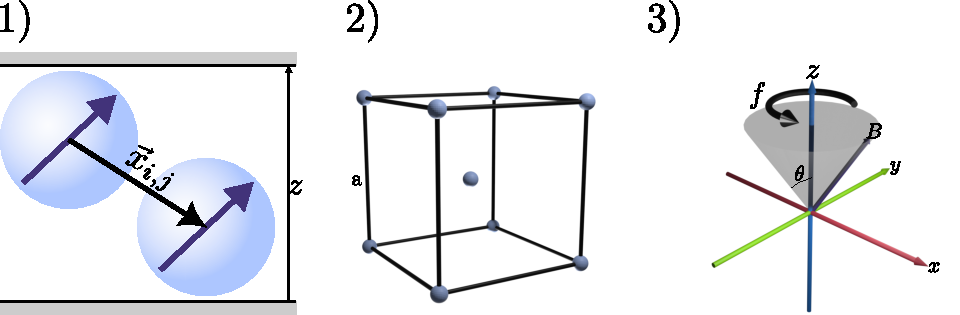
\includegraphics[width=0.95\textwidth]{figures/methods1.pdf}
  \end{center}
  \caption[Representation of the paramagnetic colloids, body-centered-cubic lattice used for the ratchet, and the precessing conic magnetic field.]{\textbf{Panel 1)} Shows two paramagnetic particles with a distance \(\vec{x}_{i,j}\) with the same dipole moment in a confined space in the \( z\) axis. \textbf{Panel 2)} Shows a representation of a  unitary body-centered cubic lattice used in the construction of the ratchet. \textbf{Panel 3} Shows the precessing external magnetic field.}\label{fig:facecenteredlattice}
\end{figure}

To model contacts, we use a Weeks-Chandler-Andersen potential (WCA), which is a LJ with only a repulsive part~\cite{hess1999augmented}:

\begin{equation}
  U_{i,j}^{WCA} = \begin{cases} 
    4\epsilon\left[ \left( \frac{\sigma}{r_{i,j}}\right)^{12} - \left( \frac{\sigma}{r_{i,j}}\right)^6\right] + \epsilon \quad &r_{i,j} \leq r_c \\
    0 \quad & r_{i,j} \geq r_c
  \end{cases}
  \label{eq:wcapotential}
\end{equation}
where $\sigma$ is the van der Waals radio, it is the point where the energy between the two particles is zero, $\epsilon$ is the well depth, since WCA does not have an attraction interaction, a correction factor of $\epsilon$ is added, and $r_c = 2^{1/6}\sigma$. This however, gives us the enegy between particles, and we need the force, then we apply:

\begin{equation}
 F = - \nabla U, 
  \label{eq:negativegradient}
\end{equation}
getting then

\begin{equation}
  F_{i,j}^{WCA} = \begin{cases} 
    48\epsilon\left[ \left( \frac{\sigma}{r_{i,j}}\right)^{12} - \frac{1}{2}\left( \frac{\sigma}{r_{i,j}}\right)^6\right]\left[ \frac{1}{r_{i,j}}\right] \quad &r_{i,j} \leq r_c \\
    0 \quad & r_{i,j} \geq r_c
  \end{cases}.
  \label{eq:wcaforce}
\end{equation}
and adding all the interaction expected by each particle, we obtain:

\begin{equation}
  F^{collision}_i = \sum^{n}_{i \neq j} F^{WCA}_{i,j}.  
  \label{eq:wcasum}
\end{equation}

We want to see how the positions of the particles evolve over time with certain initial conditions, and to solve Eq. (\ref{eq:langevindipole}) this is why we need an integration method.

\section{Euler-Maruyama Integration Method}
%%%%%%%%
The Euler-Methods is a numerical method used for stochastic differential equations which helps solve systems with Brownian motion~\cite{platen2010numerical,higham2001algorithmic}.

The overdamped Langevin equation for a particle reads
\[
\dot{\mathbf x}(t)=\mu\mathbf F(\mathbf x,t)+\sqrt{2D}\,\boldsymbol\xi(t),
\]
where \(\mu=1/\gamma\) is the mobility, \(D=k_BT/\gamma\) the diffusion coefficient,
and \(\boldsymbol\xi(t)\) is normalized Gaussian white noise:
\(\langle\xi_i(t)\rangle=0,\ \langle\xi_i(t)\xi_j(t')\rangle=\delta_{ij}\delta(t-t')\).
Discretizing with timestep \(\Delta t\) and Wiener increments \(\Delta\mathbf W\sim\mathcal N(\mathbf0, \mathbf1)\),
the Euler--Maruyama update is
\begin{equation}
\mathbf x_{n+1} = \mathbf x_n + \mu\,\mathbf F(\mathbf x_n,t_n)\,\Delta t
  + \sqrt{2D}\;\Delta\mathbf W_n.
\label{eq:em_overdamped}
\end{equation}
%%%%%%%%
\section{Definition of the Solid Ratchet}

To create the solid ratchet we used basis vectors (or lattice vectors) which are the fundamental building blocks used to generate the entire crystal lattice by translation. These vectors define the geometry of the unit cell, and by repeating the unit cell across space, we can form the overall lattice structure. Here, a body-centered cubic (BCC) lattice was chosen since the stability which proved to be stable under thermal fluctuations.
The conventional unit cell for a BCC lattice is a cube with a lattice point at each corner and one at the body center. The vectors defining this cube are simple, orthogonal, and given by:
%
\begin{equation}
  \vec{R} = m(a\hat{x}) + n(a\hat{y}) + p(a\hat{z}) + \delta \frac{a}{2}(\hat{x} + \hat{y} + \hat{z}); \quad m,n,p \in \mathbb{Z},
\end{equation}
%
where \( a \) is the lattice constant (the side length of the cube), and $\delta$ is either 0 or 1, depending if we are refering to the centered particle. Once defined the basis vectors, with help of a script we enter the required parameters that will define the size of the solid ratchet that is defined by a modulated radius function that creates $N$ teeth around the azimuthal direction. The angular coordinate $\phi \in [0, 2\pi)$ is traced in the Cartesian coordinates (x, y).
%%%%
\begin{equation}
R(\phi) = R_0 + A \cdot S\left(\frac{f\phi}{2\pi}\right) - \frac{A}{2}
\end{equation}

where $S(x)$ is the sawtooth function, $A$ is the amplitude of the sawtooth, $f$ the number of complete sawtooth cycles in the circle, $R_0$ base radius of the ratchet profile:

\begin{equation}
S(x) = \begin{cases}
1 - (x \bmod 1) & \text{Spin up} \\
x \bmod 1 & \text{Spin down}
\end{cases}
\end{equation}

Points $\mathbf{r} = (x, y, z)$ are included when $\sqrt{x^2 + y^2} \leq R(\phi)$.
However, these points must remain fixed, otherwise these would separate from each other dissolving the structure, therefore we add bonds.

There are multiple methods to model the potential energy of a bond, the easiest way is to use the harmonic potential that mimics the behavior of a ideal spring and is modeled after Hooke's law:

\begin{equation}
  U^{H}_{i,j}(\vec{x}_{i,j}) = \frac{1}{2}K(\vec{x}_{i,j} - \vec{x}_0)^2,
\end{equation}
where K is the energy per squared distance, $\vec{x}_{i,j}$ is the distance between particle \textit{i}, and \textit{j}, and $x_0$ is the equilibrium distance point.
%%%%%%%%

\section{System Overview and Workflow}

The simulations of this thesis were performed with an open-source software called LAMMPS (Large-scale Atomic/Molecular Massively Parallel Simulator) developed by Sandia National Laboratories. Its advantage is the high efficiency to run simulatios in parallel, reducing the time required to perform multiple calculations \cite{LAMMPS}. We used a modified version of LAMMPS but created custom input scripts using a Python library. These scripts will atomate the process of the input scritpts that will tell LAMMPS everything about the parameters of our simulation, such as the size of the system, the physical conditions, and how long to run for. After the simulations, we used additional custom scripts with the help of a Python library called Pandas, to analyze the results quickly and efficiently.

\begin{figure}[h]
  \begin{center}
    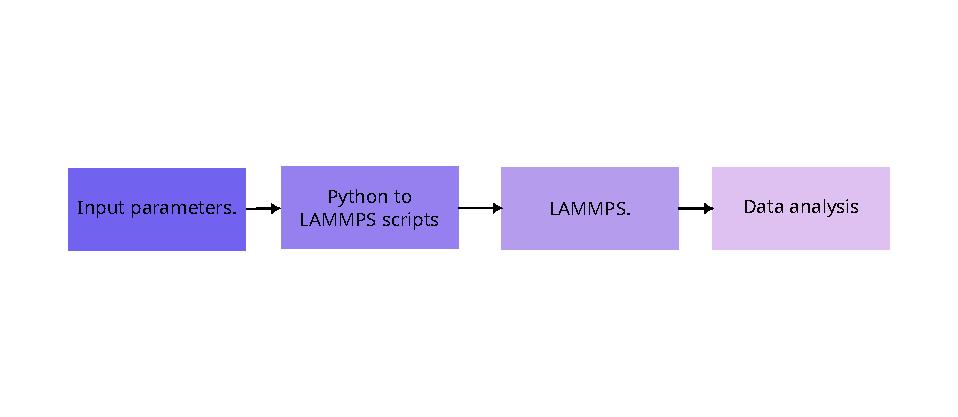
\includegraphics[width=0.95\textwidth]{figures/workflow.pdf}
  \end{center}
  \caption[Workflow diagram.]{Workflow diagram.}\label{fig:workflow}
\end{figure}

\subsection{System's Physical Definition}

The first parameters to be defined are the ones from the circular-ratchet geometry, since it will define the position of the paramagnetic colloids afterwards, these are the parameters that can be specified in the function:

\begin{table}[H]
\centering
\caption[Ratchet physical parameters.]{Parameters used for the circular ratchet in the simulation.}
\begin{tabular}{l l l l l}
\hline
Parameter & Symbol & Ratchet A & Ratchet B & Units \\
\hline
Lattice constant & \(a\) & 1 & 1 & \(\mu m\) \\
Radius & \( r\) & 8 & 8 & \( \mu m\) \\
Sawtooth amplitude & \( A\) & 4 & 4 & \( \mu m\) \\
Sawtooth frequency & \( N\) & 5 & 3 & Dimensionless\\
Bond coefficient & \( K_b\) & 0.1 & 0.1 & \( \mu N\) \\ 
Density & \(\rho\) & 1 & 1 & kgm\(^{-3}\) \\
\hline
\end{tabular}
\end{table}

\begin{figure}
  \begin{center}
    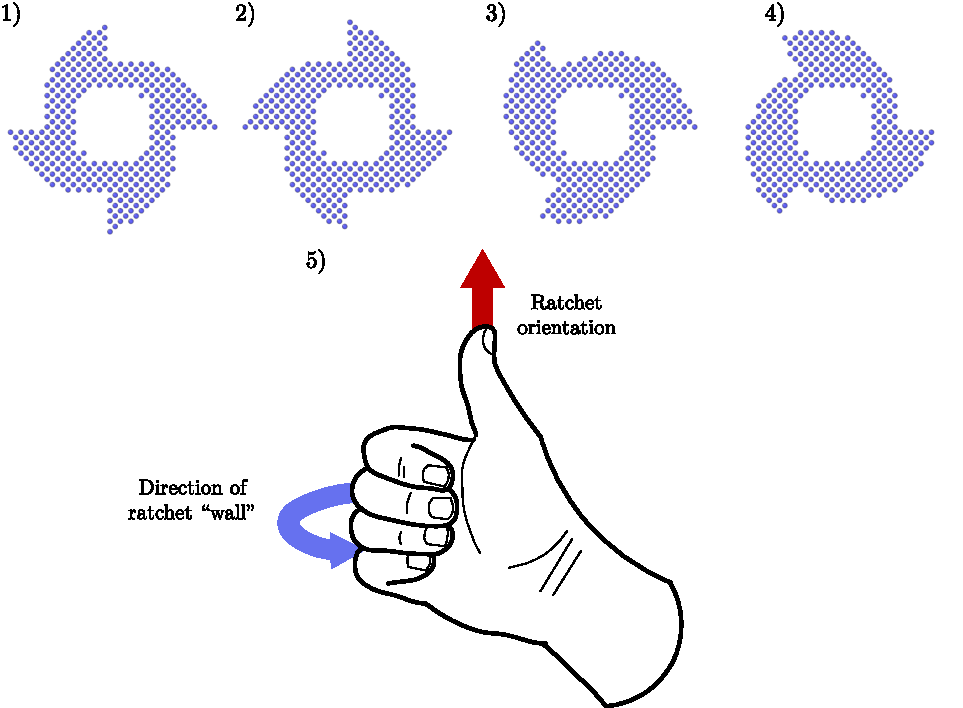
\includegraphics[width=0.95\textwidth]{figures/ratchet.pdf}
  \end{center}
  \caption[Ratchet geomety.]{Ratchet geometry used in the simulations. \textbf{Panel 1)} shows 4-spikes ratchet (Spin up).\textbf{Panel 2)} shows the same ratchet with a 180° specular rotation (Spin down). \textbf{Panel 3) - 4)} Shows the same characterisitcs with a 3-spikes ratchet. \textbf{ Panel 5)} Shows the convention used for classifying the ratchets. In this case the curl right hand rule can be used. Facing the ``wall'' of the ratchet with the palm of the hand, the thumb will indicate the geometry of the ratchet. If the thumb points towards you or upwards, the geometry will be called spin up, if it points downwards the geometry will be called spin down.}\label{fig:ratchetgeometry}
\end{figure}


As shown in the previous table, there were 2 ratchets with only a difference in te \textit{Sawtooth frequency}, but in reality we used a reflection of each ratchet for another pair of analysis. Once the ratchet geometry is defined, then we can define then the remaining of the system, which remained constant for the 2 ratchets. Starting with the simulation box, that is a rectangle box of periodic boundary conditions in axis \textit{x}, and \textit{y},and finite boundary conditions modeled with the a WCA potential:



\begin{table}[H]
\centering
\caption[Simulation box physical parameters.]{Parameters used for the box of the simulation.}
\begin{tabular}{l l l l}
\hline
Axis & lo  & hi & Units \\
\hline
\textit{x} & -27 & 27 & \( \mu m\) \\
\textit{y} & -27 & 27 & \( \mu m\) \\
\textit{z} & -2  & 2   & \( \mu m\)\\ 
\hline
\end{tabular}
\end{table}

Where \textit{lo} represent the lower boundary, an \textit{hi} the upper boundary.

Finally, the parameters for the paramagnetic particles, and since they deppend on the magnetic field, it is important to define the parameters of this one too.


\begin{table}[H]
\centering
\caption[Paramagnetic colloids parameters.]{Parameters used for the paramagnetic particles.}
\begin{tabular}{l l l l}
\hline
Parameter & Symbol  & Value & Units \\
\hline
Radius & $r_{mag}$ &  1.25 &\( \mu m\) \\
Susceptibility & $\chi$ & 0.4 & Dimensionless\\
Field angle & $\theta$ & 27 & °\\
Frequency & $f$ & [0 - 10] & Hz\\
Field magnitude & $B$ & 7.28 & mT\\
\hline
\end{tabular}
\end{table}

With these values, we can run simulations for a period of $50 \cross 10^6$ frames, with a timestep of 10 $\mu s$ which corresponds to a total real time of $500 s$ ($8.33\bar{3} \mathrm{min})$. Since these systems are of random nature, it is recommended to perform multiple simulations in order to be able to obtain reliable averaged observables, therefore we ran it 10 different times for each frequency.

\subsection{Data Analysis}

%%%%%
When a simulation is completed, LAMMPS generates a text data file containing the quantities selected for output. In this study, we are particularly interested in the particle positions of the solid object, from which several physical properties can be derived—the most relevant being the angular velocity of the ratchet.

The simulated system consists of multiple particles, each exhibiting a slightly different angular velocity due to the bond strength, which prevents them from remaining perfectly rigid with respect to one another. Consequently, it is necessary to compute an average angular velocity that represents the collective motion of all particles.

Since all particles share the same center of mass, the angular velocity can be determined by first calculating this common center, defined as follows:
%%%%%

\begin{equation}
  (x_{\mathrm{COM}}, y_{\mathrm{COM}}) = \displaystyle\frac{\sum^{n}_{i=1} m_i * r_i}{\sum^{n}_{i=1} m_i},
  \label{eq:centerofmass}
\end{equation}
being $m_i$ the mass of the particle \textit{i}, and $r_i$ the position of the particle respect a frame of reference. The best way to calculate the angular velocity is by using polar coordinates, once we have the center of mass, we convert the positions to polar coordinates:

\begin{align}
  r_i & = \sqrt{(x - x_{\mathrm{COM}})^2 + (y - y_{\mathrm{COM}})^2},\\ 
  \theta _i &= \arctan{\frac{y - y_{\mathrm{COM}}}{x - x_{\mathrm{COM}}}},
\end{align}
then we can calculate the angular velocity of each particle for each timestep of the simulation:
\begin{equation}
  \omega _i = \frac{\Delta \theta _i}{\Delta t},
  \label{eq:angularvelocity}
\end{equation}

then obtaining an average angular velocity of all particles. We average over all particles to obtain the angular velocity of the solid object.

 \newpage
\part{Results}
\label{part:results}

\chapter{Results}

\begin{figure}
  \begin{center}
    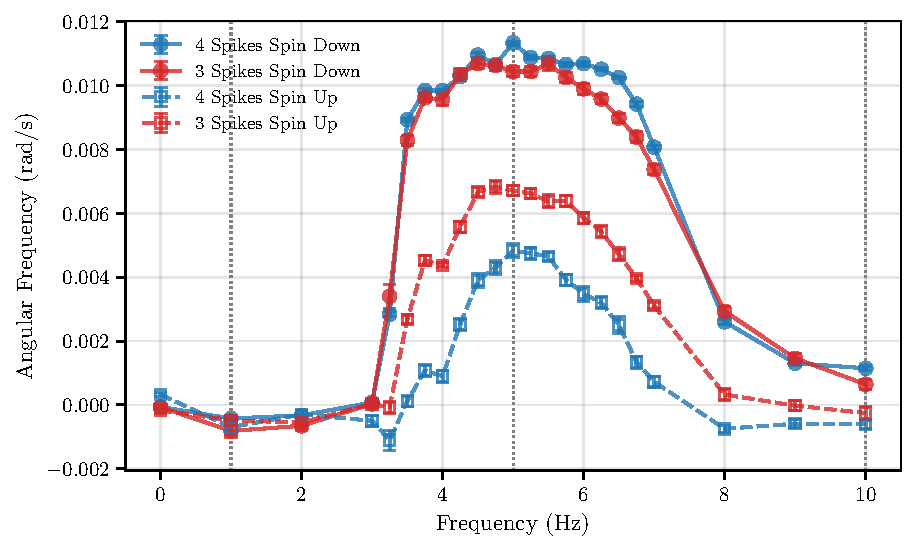
\includegraphics[width=0.95\textwidth]{figures/AvsF.pdf}
  \end{center}
  \caption[Angular velocity graph.]{Angular velocity vs Frequency}\label{fig:angularvsfrequency}
\end{figure}

\begin{figure}
  \begin{center}
    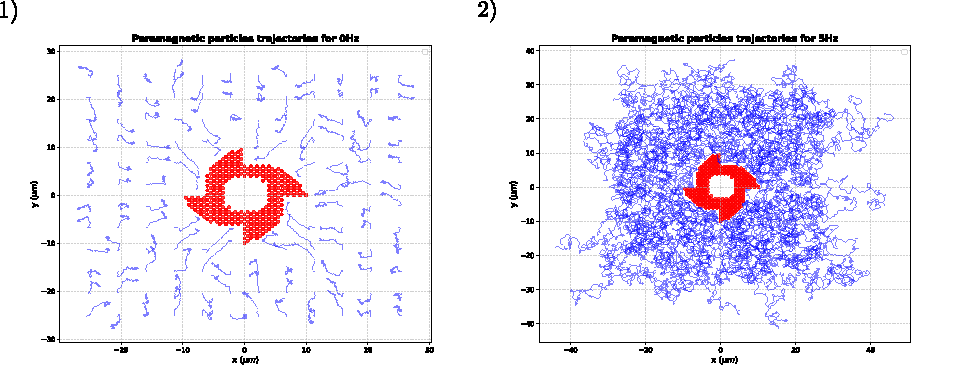
\includegraphics[width=0.95\textwidth]{figures/particlesTrj.pdf}
  \end{center}
  \caption[Particles trajectories]{Particles trajectories from 0 to 1e10 frames for 0Hz.}\label{fig:particletrj}
\end{figure}

\begin{figure}
  \begin{center}
    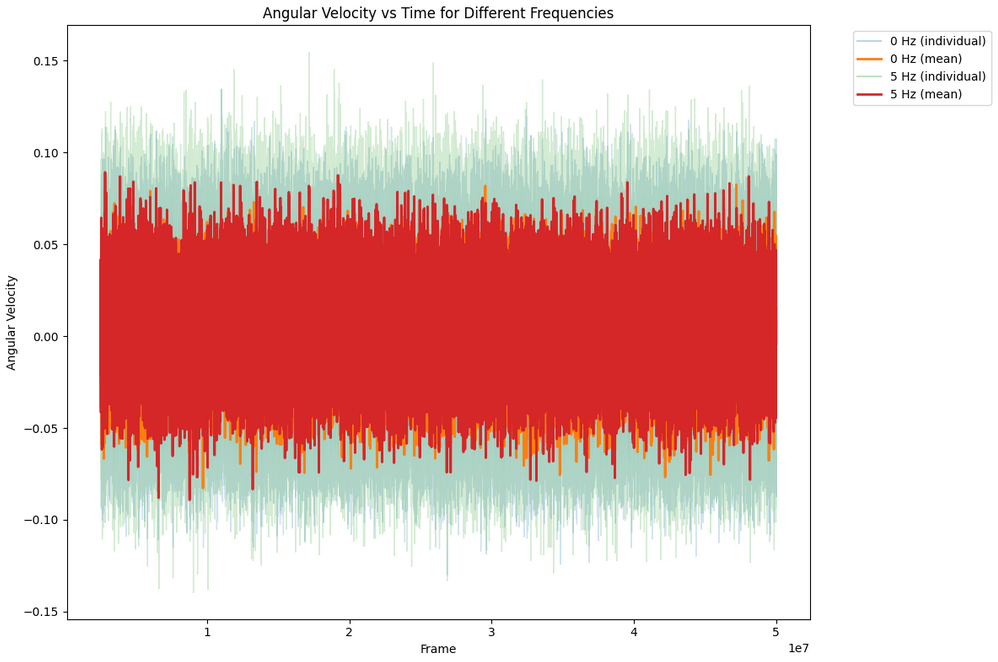
\includegraphics[width=0.95\textwidth]{figures/velocityVsTime.png}
  \end{center}
  \caption{}\label{fig:velocityvstime}
\end{figure}


 \newpage
\part{Conclusions}
\label{part:conclusions}

\chapter{Conclusions}

We have seen how motion at small scales becomes difficult due to the increase in the relative viscosity of fluids, which suppresses inertia and makes displacement dependent the available degrees of freedom. Random forces, known as thermal fluctuations, also play an important role by constantly disturbing the motion of particles. Nevertheless, both theory and experiments have shown that even passive particles can achieve rectified motion when subjected to specific asymmetric conditions. In this thesis, we focused on ratchet effects, particularly those observed under optically generated potential landscapes.

We also discussed advances in artificial active particles, while emphasizing natural systems. These biological microswimmers demonstrate how energy can be converted into motion and even into useful work, giving rise to micromachines capable of transporting objects or generating rotation through chemical or biological activity. However, these systems face practical limitations: they are prone to biological degradation and require a continuous source of energy to remain active.

As an alternative, we discussed magnetically driven environments, focusing on spherical paramagnetic colloids driven by an external magnetic field. Experimental studies have already demonstrated that it is possible to rectify the motion of such particles, typically using ferrite garnet films to generate the required asymmetry. Yet, there also exist examples where directed motion is achieved without these substrates, relying only on a conical magnetic field.

In this thesis, we explored the effects of a conical external magnetic field on a solid ratchet immersed in paramagnetic spherical colloids suspended in water and confined geometry. The system was studied using Brownian and molecular dynamics simulations. We analyzed physical quantities such as angular displacement and angular velocity, as they are key indicators of motion rectification.

Our analysis suggests that in the frequency range of 3.25–8 Hz there is a noticeable increase in angular velocity, which remains roughly constant—though with some fluctuations—between 3.75 and 7.75 Hz. This indicates partial rectification of motion. Although the effect is not strong enough to produce complete rotations within short timescales, it opens a new line of research to enhance the efficiency of this type of system. The same behavior was observed for all four ratchet configurations studied. Interestingly, when the ratchet geometry was rotated by 180°, the overall direction of rotation remained unchanged, even though the ratchet walls were mirrored. This raises an open question about whether the rotation can be controlled through geometry or if it depends entirely on the external magnetic field.

To ensure the accuracy of these results, we performed additional analyses on individual datasets using a moving mean filter, and histogram for the lowest (0 Hz) and highest (5 Hz) frequencies. These results confirmed the overall behavior observed in the averaged data and validated our main findings.

In summary, we explored how it is possible to obtain work from passive environments when induced in a assymetric potentials in non-symmetric objects. This thesis opens to discussion about how other parameters of the geometry of the ratchet can effectively affect the rotation of it, such as the radius, wall length, a lower or bigger amount of \textit{spikes}, a bigger amount of colloids, different colloids radius. 
 \newpage

%----- END MATERIAL -----%

% Appendices-----------------------------------------------------------

% \appendix
%
%%======================================================================
\chapter{Name of Appendix}
\markright{Name of Appendix} % new right header
%======================================================================

Uso de referencias \cite{Moody92} and \cite{Sjoberg95}
\newpage

%%======================================================================
\chapter{Diagnosis in Dynamic Systems}
\label{app2:diadynsys}

\markright{Diagnosis in Dynamic Systems}
%======================================================================

\section {Definitions}
\label{app2:SysDefinitions}

Some important definitions in dynamic systems are:
\begin{enumerate}
\item \emph{Static versus dynamic systems.} \\  A system is \item
\emph{Linear versus non-linear models.} \\ A linear model,
\end{enumerate}

\section {The Qualitative Model Representation}
\label{app2:quarea}

\newpage


%
% References-----------------------------------------------------------
\markright{Bibliography}
\addcontentsline{toc}{chapter}{Bibliography}
\bibliographystyle{unsrtnat} % in order of appearance
\bibliography{references.bib}

% Index ---------------------------------------------------------------

\printindex

\huge{Curriculum Vitae} \\
\addcontentsline{toc}{chapter}{Curriculum Vitae}
\markright{Curriculum Vitae} % new right header
\normalsize
\vspace*{1.0 cm}


\emph{Yeray Cruz Ruiz} was born in Tlalnepantla, Estado de México, México. He received a Bachelor of Science degree in Mechatronics (2021) from Tecnológico de Monterrey, Campus Monterrey, México, where he is currently a full-time master's student in Nanotechnology, focusing on computational studies of soft matter systems out of thermodynamic equilibrium. His research interests include Soft Matter Physics, Colloidal Models, Passive Matter, and Active Matter,  and Computational Physics. 



\end{document}
%======================================================================
